\documentclass[aspectratio = 169]{beamer}

\usepackage[utf8]{inputenc} % Character encoding.

\pdfinfo{
   /Author (Bashar Dudin)
   /Title  (The Simplex Algorithm I)
   /Subject (Linear Programs)
}


\usepackage{./Style/linearProgramsBeamer} % This is extra styling for Beamer environments.
\usepackage{./Style/linearProgramsStyle} % This is a set of commands for maths content.

%-------------------------------------------------------------------------------
%   TITLE PAGE
%-------------------------------------------------------------------------------

\author[BD]{Bashar Dudin}

\institute[]{EPITA}

\title{Programmes linéaires} %
\subtitle{Algotithme du simplexe I}

%-------------------------------------------------------------------------------
%   DOCUMENT BODY
%-------------------------------------------------------------------------------

\begin{document}

\begin{frame}[plain]
\titlepage % Print the title page as the first slide
\end{frame}

\section{Optimisation linéaire sous contraintes polyédrales}

\begin{frame}{Géométrie de l'espace admissible}
  On considère le programme linéaire $L$ dans sa forme standard:
    \begin{figure}
        \begin{linearProg}{
            maximiser
            }{
            $x_1 + 2x_2$
            }{
            \systeme{x_1 + x_2 \leq 5, -2x_1 + x_2 \leq 3}
            }{
            $x_1, x_2 \geq 0$
            }
        \end{linearProg}
    \end{figure}
    L'ensemble des solutions admissibles de $L$ est la région du plan
    dans le premier cadran délimité par les équations $x_2 = 5 - x_1$
    and $x_2 = 3 + 2x_1$.
\end{frame}

\begin{frame}{Géométrie de l'espace admissible}
  \begin{columns}
    \begin{column}{.5\textwidth}
      L'ensemble des solutions admissibles de $L$ jouit d'une
      propriété remarquable qu'on appelle la \textit{convexité}.
      \pause
      \begin{defn}
        Un sous-ensemble $A$ de $\R^n$ est dit \emph{convexe} si tout
        segment qui relie deux points quelconques de $A$ est inclus
        dans $A$.
      \end{defn}
      \pause
      Dans les cas des programme linéaire on travaille avec un cas
      particulier des parties convexes appelée \emph{polyèdre}. C'est
      une intersection de demi-espaces.
    \end{column}
    \begin{column}{.6\textwidth}
      \begin{figure}
        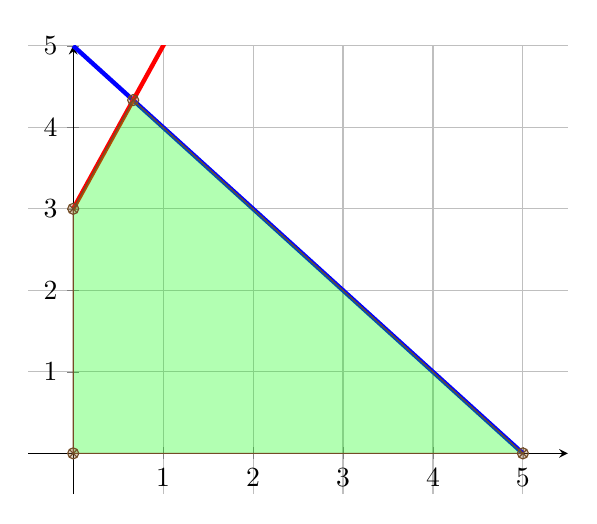
\begin{tikzpicture}
          \begin{axis}[
            domain=0:5, xmin=-0.5, xmax=5.5, ymin=-0.5, ymax=5,
            grid=major, axis x line=center, axis y line=center,
            legend pos=north east,
            ]
            \addplot+[ultra thick, mark = none] {5 - x};
            \addplot+[ultra thick, mark = none] {3 + 2*x};
            \addplot+[fill = green, fill opacity = 0.3] coordinates
            {(0,0) (0,3) (.667,4.334) (5,0)} \closedcycle ;
          \end{axis}
        \end{tikzpicture}
      \end{figure}
    \end{column}
  \end{columns}
\end{frame}

\begin{frame}{Géométrie de l'espace admissible}
  \begin{prop}
    Un programme linéaire a un espace admissible sous-jacent qui est
    convexe.
  \end{prop}
  \begin{defn}
    On appelle \emph{intérieur} d'une partie convexe $A$ l'ensemble
    des points $x \in A$ pour lesquels il existe un \textit{disque} de
    rayon strictement positif centré en $x$ et contenu dans $A$. Tout
    point de $A$ qui ne satisfait cette condition est appelé un
    \emph{point du bord}. Le \emph{bord} de $A$ est l'ensemble des
    points du bord (potentiellement vide).
  \end{defn}
  Les points du bord d'un polyèdre (défini par des contraintes
  linéaires), se situent sur les hyperplans obtenus en rempla\c{c}ant
  les inégalités des contraintes par des égalités. C'est clairement le
  cas dans notre exemple bidimensionnel.
\end{frame}

\begin{frame}{Les points optimaux sont des points du bord}
  On rappelle qu'une fonction $f : A \to \R$ est dite \emph{bornée}
  s'il existe un réel positif $M$ tel que: pour tout $x \in A$,
  $\big|f(x)\big| \leq M$.
  \begin{prop}
    Soit $A$ l'espace admissible d'un programme linéaire $L$. Si la
    fonction objectif est \textit{bornée} sur $A$ alors $L$ a une
    valeur optimale et elle atteinte sur le bord de $A$ (si non vide).
  \end{prop}
  La justification de ce résultat en dit bien plus!
\end{frame}

\begin{frame}{Les points optimaux sont des points extrémaux}
  Soit $A$ l'espace admissible d'un programme linéaire $L$, supposé
  écrit sous forme standard. Un \emph{point extrémal} de $A$ est un
  point $x$ pour lequel tout \textit{disque} centrée en $x$ ne
  contient aucun segment (ouvert) centré en $x$ et contenu dans
  $A$. \pause

  De tels points sont nécessairement des points du bord de
  $A$ ; ils apparaissent comme des intersections d'autant d'hyperplan
  que la dimension du programme. \pause
  \begin{prop}
    Si la fonction objectif d'un programme linéaire $L$ est bornée sur
    $A$ alors $L$ a une valeur optimale atteinte en un point extrémal
    de $A$ (s'il y en a un).
    \end{prop}
\end{frame}

\begin{frame}{Les points optimaux sont des points du bord | Recherche Naive}
  Soit $L$ un programme linéaire de dimension $n$. Une approche naive
  pour rechercher les points optimaux est d'étudier l'ensemble des
  points extrémaux de $L$, et d'y comparer les valeurs
  objectifs.
  \pause

  Recercher un point extrémal revient à résoudre un
  système linéaire ayant $n$ équations.
  \pause
  \begin{halfshyblock}{Question}
    Soit $n \in \N^*$. On consdière les contraintes linéaires
    \[
      \forall i \in \{1, \ldots, n\}, \quad 0 \leq x_i \leq 1.
    \]
    Quel est le nombre de points extrémaux que définissent ces
    contraintes?
  \end{halfshyblock}
  \pause Comme le montre cet exemple, la complexité au pire est
  exponentiellement proportionnelle au nombre de contraintes
  linéaires.
\end{frame}

\begin{frame}{Les points optimaux sont des points du bord | Une meilleure recherche}
  Au lieu de lister tous les points optimaux potentiels, l'algorithme
  du \emph{simplexe} est une marche le long des points extrémaux de
  l'espace admissible qui vérifie la propriété :
  \begin{quotation}
    Une itération du \emph{simplexe} renvoie uen valeur objectif plus
    grande que la précédente.
  \end{quotation}
  \pause Le simplexe nécessite une étape d'initialisation qu'on laisse
  de côté pour l'instant en travaillant sous l'hypothèse suivante:
  \begin{alertblock}{Hypothèse}
    Étant donné un programme $L$ sous forme \textit{standard}, on
    suppose que le vecteur nul est admissible.
  \end{alertblock}
  \pause Dans l'exemple à venir, en commen\c{c}ant par la solution
  nulle on marche le long des points extrémaux pour chercher la valeur
  optimale.
\end{frame}

\section{Algorithme du simplexe : premier essai}

\begin{frame}{Algorithme du simplexe : premier exemple pratique}
  Voici la forme \textit{slack} du programme $L$ de départ:
    \begin{figure}
      \begin{linearProg}{
          maximiser
        }{
          $x_1 + 2x_2$
        }{
          \systeme{x_3 = 5 - x_1 - x_2, x_4 = 3 + 2x_1 - x_2 }
        }{
          $x_1$, $x_2$, $x_3$, $x_4 \geq 0$
        }
      \end{linearProg}
    \end{figure}
    La solution admissible nulle de la forme standard de $L$
    correspond à la solution $(0, 0, 5, 3)$ de cette forme-ci ; elle
    est de valeur objectif nulle. Les variables d'écarts $x_3$ et
    $x_4$ quantifie ô combien la solution $(x_1, x_2)$ est loin de
    faire des inégalités
    \[
    \sysdelim..{\systeme{x_1 + x_2 \leq 5, -2x_1 + x_2 \leq 3}}
    \]
    des égalités.
\end{frame}

\begin{frame}{Algorithme du simplexe : premier exemple pratique}
    \begin{columns}
        \begin{column}{.5\textwidth}
          \begin{onlyenv}<1
            >La soluion \textit{slack} $(0, 0, 5, 3)$
            a une solution \textit{standard} l'origine du plan. Pour
            se balader le long du bord du lieu admissible on doit
            choisir par où aller ; verticalement laissant $x_1$ à $0$
            ou horizontalement avec $x_2$ à $0$. Tout choix est bon
            tant qu'on augmente la valeur objectif. On sera plus
            précis sur ce choix plus tard. Pour l'instant on choisit
            d'augmenter $x_1$, $x_2$ restant constant.
            \end{onlyenv}
            \begin{onlyenv}<2
              >
              \begin{figure}
                \small{
                  \begin{linearProg}{
                      maximiser
                    }{
                      $x_1 + 2x_2$
                    }{
                      \systeme{x_3 = 5 - x_1 - x_2@(E_{*}), x_4 = 3 + 2x_1 - x_2 }
                    }{
                      $x_1$, $x_2$, $x_3$, $x_4 \geq 0$
                    }
                  \end{linearProg}
                }
              \end{figure}
              $x_1$ est contrainte par $E_1$: l'augmenter indéfiniment
              violerait les contrainte de positivité. Il n'y a pas de
              telle contrainte de $E_2$. La plus grande valeur
              possible pour $x_1$ est donc obtenue quand $x_3$ vaut
              $0$. La solution obtenue ainsi est $(5, 0, 0, 13)$ de
              valeur objectif $5$. Elle satisfait l'égalité definie
              par la première contrainte.
            \end{onlyenv}
            \begin{onlyenv}<3
              >
              \begin{figure}
                \small{
                  \begin{linearProg}{
                      maximiser
                    }{
                      $x_1 + 2x_2$
                    }{
                      \systeme{x_3 = 5 - x_1 - x_2@(E_{*}), x_4 = 3 + 2x_1 - x_2 }
                    }{
                      $x_1$, $x_2$, $x_3$, $x_4 \geq 0$
                    }
                  \end{linearProg}
                }
              \end{figure}
              La solution $(0, 0, 5, 3)$ peut être comprise comme
              mettant $x_1$ et $x_2$ à $0$. Pour $(5, 0, 0, 13)$ il
              s'agit d'en faire autant pour $x_3$ et $x_2$. \pause Ce
              fait est général : un point extrémal correspond au cas
              où $2$ variables exactement sont à $0$. \pause Pour
              conserver la pattern \textit{annuler une variable à
                gauche} on échange $x_1$ et $x_3$ de côtés.
            \end{onlyenv}
            \begin{onlyenv}<4
              >Pour obtenir la solution $(5, 0, 0, 13)$ on peut
              exprimer $x_1$ dans $E_1$ en fonction du reste. Cette
              expression remplace $x_1$ dans les autres contraintes.
              D'où le programme équivalent
                \begin{figure}
                  \small{
                    \begin{linearProg}{
                        maximiser
                      }{
                        $5 - x_3 + x_2$
                      }{
                        \systeme{x_1 = 5 - x_3 - x_2@(E_{*}), x_4 = 13 - 2x_3 - 3x_2 }
                      }{
                        $x_1, x_2, x_3, x_4 \geq 0$
                      }
                    \end{linearProg}
                  }
                \end{figure}
                Si l'on annule $x_3$ et $x_2$ on retrouve la solution
                admissible attendue.
            \end{onlyenv}
            \begin{onlyenv}<5-6
                >\alt<5>{
                \textcolor{orange}{
                \begin{figure}
                  \small{
                    \begin{linearProg}{
                        maximiser
                      }{
                        $\dfrac{28}{3} - \dfrac{5}{3}x_3 - \dfrac{1}{3}x_4$
                      }{
                        \systeme{x_1 = 2/3 - (1/3)x_3 + (1/3) x_4@(E_{*}), x_2 = 13/3 - (2/3)x_3 - (1/3)x_4 }
                      }{
                        $x_1$, $x_2$, $x_3$, $x_4 \geq 0$
                      }
                    \end{linearProg}
                  }
                \end{figure}
              } \vspace{-1em}
              En réitérant la démarche précédente avec $x_2$ et la
              seconde équation on obtient le programme ci-dessus. En
              mettant $x_3$ et $x_4$ à $0$, on obtient une valeur
              objectif de $28/3$.  }{
                \begin{figure}
                  \small{
                    \begin{linearProg}{
                        maximiser
                      }{
                        $5 - x_3 + x_2$
                      }{
                        \systeme{x_1 = 5 - x_3 - x_2@(E_{*}), x_4 = 13 - 2x_3 - 3x_2 }
                      }{
                        $x_1$, $x_2$, $x_3$, $x_4 \geq 0$
                      }
                    \end{linearProg}
                  }
                \end{figure}
                On peut espérer augmenter la valeur objectif via
                $x_2$. Toute augmentation de $x_3$ donnerait une plus
                petite valeur objectif. L'équation la plus restrictive
                pour $x_2$ est $E_2$.  }
            \end{onlyenv}
            \begin{onlyenv}<7->
                \begin{figure}
                  \small{
                    \begin{linearProg}{
                        maximiser
                      }{
                        $\dfrac{28}{3} - \dfrac{5}{3}x_3 - \dfrac{1}{3}x_4$
                      }{
                        \systeme{x_1 = 2/3 - (1/3)x_3 + (1/3) x_4@(E_{*}), x_2 = 13/3 - (2/3)x_3 - (1/3)x_4 }
                      }{
                        $x_1$, $x_2$, $x_3$, $x_4 \geq 0$
                      }
                    \end{linearProg}
                  }
                \end{figure}
                \vspace{-1em}
                On ne peut, désormais, plus espérer augmenter la
                valeur objectif. Tout augmentation de $x_3$ ou $x_4$
                diminuerait la valeur objectif. La valeur objectif
                maximal serait donc $28/3$, atteinte en
                $(2/3, 13/3, 0, 0)$.
            \end{onlyenv}
        \end{column}
        \begin{column}{.5\textwidth}
            \begin{overlayarea}{\textwidth}{.8\textheight}
                \begin{onlyenv}<1>
                \begin{figure}
                    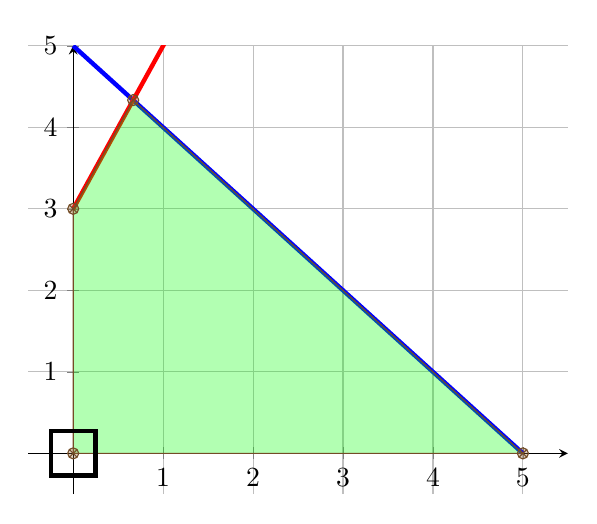
\begin{tikzpicture}
                        \begin{axis}[
                            domain=0:5, xmin=-0.5, xmax=5.5, ymin=-0.5, ymax=5,
                            grid=major, axis x line=center, axis y line=center,
                            legend pos=north east,
                            ]
                            \addplot+[ultra thick, mark = none] {5-x};
                            \addplot+[ultra thick, mark = none] {3 + 2*x};
                            \addplot+[fill = green, fill opacity = 0.3] coordinates
                            {(0,0) (0,3) (.667,4.334) (5,0)} \closedcycle ;
                            \addplot[ultra thick, black, mark size = 8pt, mark = square] coordinates {(0,0)};
                        \end{axis}
                    \end{tikzpicture}
                \end{figure}
                \end{onlyenv}
                \begin{onlyenv}<2-5>
                    \begin{figure}
                    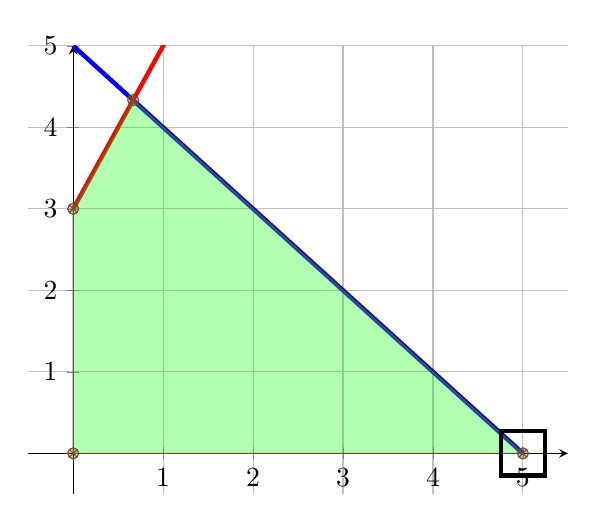
\begin{tikzpicture}
                        \begin{axis}[
                            domain=0:5, xmin=-0.5, xmax=5.5, ymin=-0.5, ymax=5,
                            grid=major, axis x line=center, axis y line=center,
                            legend pos=north east,
                            ]
                            \addplot+[ultra thick, mark = none] {5-x};
                            \addplot+[ultra thick, mark = none] {3 + 2*x};
                            \addplot+[fill = green, fill opacity = 0.3] coordinates
                            {(0,0) (0,3) (.667,4.334) (5,0)} \closedcycle ;
                            \addplot[ultra thick, black, mark size = 8pt, mark = square] coordinates {(5,0)};
                        \end{axis}
                    \end{tikzpicture}
                \end{figure}
                \end{onlyenv}
                \begin{onlyenv}<6->
                    \begin{figure}
                    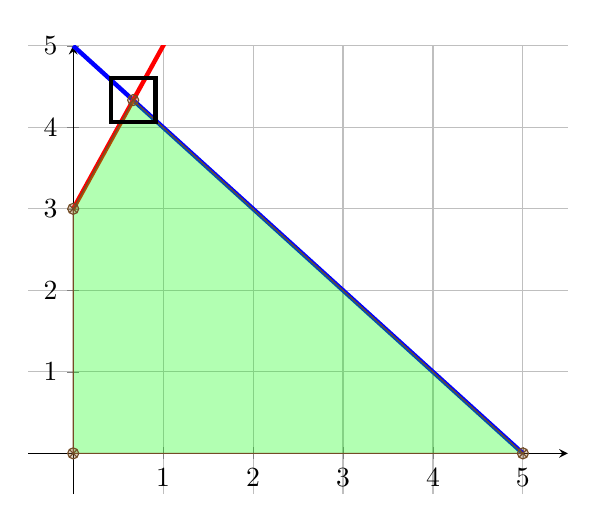
\begin{tikzpicture}
                        \begin{axis}[
                            domain=0:5, xmin=-0.5, xmax=5.5, ymin=-0.5, ymax=5,
                            grid=major, axis x line=center, axis y line=center,
                            legend pos=north east,
                            ]
                            \addplot+[ultra thick, mark = none] {5 - x};
                            \addplot+[ultra thick, mark = none] {3 + 2*x};
                            \addplot+[fill = green, fill opacity = 0.3] coordinates
                            {(0,0) (0,3) (.667,4.334) (5,0)} \closedcycle ;
                            \addplot[ultra thick, black, mark size = 8pt, mark = square] coordinates {(.667, 4.334)};
                        \end{axis}
                    \end{tikzpicture}
                    \end{figure}
                \end{onlyenv}
            \end{overlayarea}
        \end{column}
    \end{columns}
\end{frame}

\section{Algorithme du simplexe : un peu de formalisation}

\begin{frame}{Notation et terminologie}
  On considère le programme donné sous forme standard par
  \begin{figure}
    \begin{linearProgG}{
        ${\displaystyle z = \nu + \sum_{j=1}^n c_jx_j}$
      }{
        ${\displaystyle \forall i \in \{ 1, \ldots, m \}, \quad \sum_{j=1}^n a_{ij}x_j \leq b_i}$
      }{
        $\forall j \in N, \quad x_j \geq 0$
      }
    \end{linearProgG}
  \end{figure}
  L'ensemble $N$ est l'ensemble $\{ 1, \ldots, n \}$ des indices de
  variables. Notez que $\nu$ est la valeur objectif de la solution de
  base ; ce n'est pas une solution admissible en général, elle peut
  avoir des entrées négatives.
\end{frame}

\begin{frame}{Notation et terminologie}
  La forme \textit{slack} du programme précédent s'écrit
  \begin{figure}
    \begin{linearProgG}{
        ${\displaystyle z = \nu + \sum_{j=1}^n c_jx_j}$
      }{
        ${\displaystyle \forall i \in \{1, \ldots m \}, \quad x_{i + n} = b_i - \sum_{j=1}^n a_{ij}x_j}$
      }{
        $\forall j \in N\cup B, \quad x_j \geq 0$
      }
    \end{linearProgG}
  \end{figure}
  L'esnsemble des variables indexées par
  $B = \{n + 1, \ldots, n + m \}$ (à gauche) sont dites de
  \emph{base}. Les variables indexées par $N$ (à droite) sont dites
  \emph{hors base}. La \emph{solution de base} d'un tel programme est
  obtenue en mettant toutes les variables hors bases à $0$.
\end{frame}

\begin{frame}{Meta-étapes du simplexe}
  L'hypothèse temporaire sous laquelle nous travaillons peut être
  phrasée comme suit:
  \begin{alertblock}{Hypothèse (BF)}
    La solution de base du programme initiale sous-forme standard est
    admissible.
  \end{alertblock}
  Sous cette hypothèse aucun prétraitement n'est nécessaire pour
  lancer les pivots du simplexe. On traite en un premier temps le cas
  satisfaisant (\emph{BF}), avant d'attaquer le cas général.
\end{frame}

\begin{frame}{Méta-étapes du simplexe}
  Le simplexe est une série d'opérations pivots échangeant une
  variable de base avec une autre hors-base.\pause En voici les étapes
  essentielles sous (\emph{BF}).
  \begin{itemize}
  \item<2->[\textbullet] Choisir une variable hors-base $x_e$ qui
    augmente la valeur objectif.
  \item<3->[\textbullet] Utiliser la contrainte la plus
    restrictive$\ell$ sur $x_e$ pour exprimer $x_e$ en fonction du
    reste.
  \item<4->[\textbullet] Remplacer $x_e$ dans le reste des équations
    et la fonction objectif par l'expression précédente. La variable
    $x_e$ devient de base et la variable $x_\ell$ hors-base.
  \item<5->[\textbullet] En mettant toutes les variables hors-base à
    $0$ on obtient un tuple dont les $n$ premières entrées forment une
    solution admissible de notre programme linéaire.
  \item<6->[\textbullet] Réitérer les étapes précédentes jusqu'à ne
    plus pouvoir augmenter la valeur objectif.
  \end{itemize}
\end{frame}

\begin{frame}{KO sur la non bornitude\footnote{Du verbe bornituder.}}
  Il n'y aucune garantie que l'algorithme précédent nous donne bien la
  valeur optimale du programme de départ. On sait, en général, que si
  la fonction objectif est bornée sur la région admissible, alors il y
  a une valeur optimale atteinte sur le bord de cette région. Il y a
  cependant des cas où un programme linéaire n'a pas une fonction
  objectif bornée sur le l'espace admissible.
  \begin{halfshyblock}{Non bornitude}
    Trouver un programme linéaire qui n'est pas borné!
  \end{halfshyblock}
\end{frame}

\begin{frame}{Méta-étapes du simplexe}
  Les étapes précédentes sont précisément ce qu'on a effectué lors de
  l'étude de notre premier exemple. Cette approche ne se limite
  cependant pas au de dimension $2$.
  \begin{halfshyblock}{Un cas de dimension $3$}
    En suivant la démarche précédente, tenter de résoindre le
    programme suivant:
    \begin{figure}
      \begin{linearProg}{
          maximiser
        }{
          $3x_1 + x_2 + 2x_3 $
        }{
          \systeme{x_1 + x_2 + 3x_3 \leq 30, 2x_1 + x_2 + 5x_3 \leq 24, 4x_1 + x_2 + x_3 \leq 36}
        }{
          $x_1, x_2, x_3 \geq 0 $
        }
      \end{linearProg}
    \end{figure}
  \end{halfshyblock}
\end{frame}

\begin{frame}
  \begin{center}
    {\huge \textbf{C'est tout pour aujourd'hui!}}
  \end{center}
\end{frame}



%%%%%%%%%%%%%%%%%%%%%%%%%%%%%%%%%%%%%%%%%%%%%%%%%%%%%%%%%%%%%%%

\end{document}


%%% Local Variables:
%%% mode: latex
%%% TeX-master: t
%%% End:
